\section{How to Analyze Usage Data}

The tools described in this chapter provide the usage data you can use to study developer interactions, but leave the selection of methods for analyzing the data to the reader.  In this section we discuss several data analysis techniques that you may apply to usage data.  We will discuss attributes of the data including format and anonymity of the data, categorizing the records, defining sequences, using state models, and other techniques to extract information from the usage data. 

\label{sec:dataAnonymity}
\subsection{Data Anonymity}

\noindent
{\bf Non-anonymous data}, where sensitive information including source code snippets, change-sets, and even access to the source code base is provided has obvious advantages. We can replay developers' activity stream, affording them a deep understanding of the developer's actions~\citeaffixed{VakilianETAL2012UseDisuseMisuse}{e.g.,}. There are few limits on how this data can be analyzed, and {\em non-anonymous data is well-suited for exploratory studies}. Unfortunately, there are some key disadvantages. First, it may not be permitted for developers to participate in a study; typical enterprise developers may face termination if they were to leak even parts of their source code base. Second, while playback and other deep analyses are possible, these analyses can be costly in terms of time and resources. 

\vspace{0.1in}

\noindent
{\bf Anonymous data}, where only records of activities and anonymous facts about artifacts are recorded, may at first seem strictly inferior. Indeed there are some limitations on what can be learned from anonymous activity streams, yet there are key advantages. First,~\citeasnoun{SnipesExperiencesGamifyingSoftwareDevelopment} report that developers are more receptive to sharing anonymous data, and thus the ability to collect a large amount of information from many developers increases greatly. Second, because the data set is relatively large and is harvested from working developers, conclusions are ultimately more reliable. 

In this section we focus on analyzing anonymous data sources. We do so because analyzing anonymous activity streams is similar to analyzing non-anonymous data streams (i.e., they are both activity streams) and because the unlimited variation of analysis permitted by non-anonymous data affords few generalities. As we discuss analyzing usage data we start with straightforward magnitude analysis, build to a categorization system for activity streams, discuss dividing streams into sessions, and finally state-based analysis. 

\subsection{Usage Data Format}

Most usage data is collected as an activity stream with varying levels of supporting detail. In Figure~\ref{fig:theoretical} we present an abstraction of a typical activity stream. It includes a time-stamp, followed by the activity, appended with (often anonymous) details concerning that activity. We can apply this model to the examples discussed earlier. For instance, the Mylyn Monitor's interaction event corresponds to a row in our theoretical model. It includes a time-stamp (i.e., StartDate), an activity description (i.e., Kind, OriginId), and additional information (i.e., StructureHandle, StructureKind). Similarly, the CodingSpectator example includes a time-stamp (i.e., stamp), an activity description (i.e., id), and a much larger set of additional information (i.e., code-snippet, selection, selection-in-code-snippet, etc.). Because these and other usage data activity streams can easily be described using our abstraction we will refer to it as we describe data analysis techniques.


%TODO: Rewrite/Adapt/Remove this paragraph now that it's been integrated

%What do they look like

%include theoretical example

%several concrete examples (codingsepctator, Sando, Eclipse study)

%Software systems often keep a record about what event was completed (or not) in the form of a log file. The information collected in the log file is often used for diagnostic purposes. If a system failure occurs, the logs for that period can be inspected to see which sequence of events were executed by the system and what were the values for the dynamic information in those events. Each log line can be traced back to a particular line of code where the method to log this information was called. Hene, we can get complete information on what events were executed. The log message store information about the branches taken by that particular instance of execution and the values for variables in the code. Due to these reasons, the information in the log file is collected as a serially ordered flat text file. In short, a log file is a collection of log lines, with each of them having information about a single event, its time of execution and the dynamic information about variable values. Note that each log line may span across multiple lines, but provides information to distinct two adjacent log lines.



\begin{figure*}[t]
 \centering
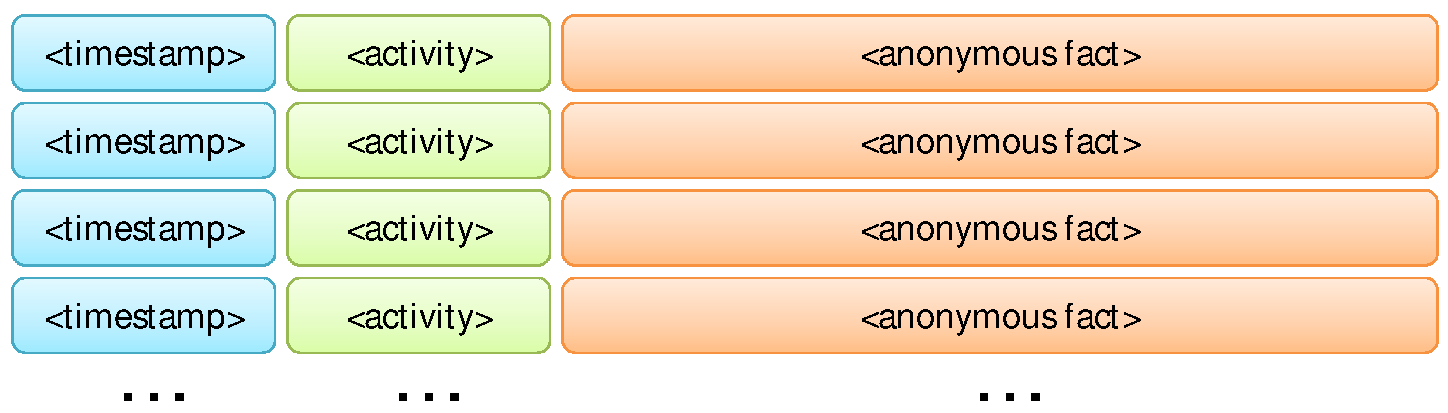
\includegraphics[width=1\columnwidth]{26Snipes_activityLogTheoretical.pdf}
\caption{Abstract model of developer activity streams.}
\label{fig:theoretical}
\end{figure*}



\subsection{Magnitude Analysis}

%advantages
A major advantage of anonymous usage data is the fact that it captures developers in their natural habitat, without any observational bias. Deriving conclusions from hours of developers' field work is naturally more convincing than from hour-long, in-laboratory developer studies. One type of questions that usage data is well-suited to answer uses measurement of the magnitude of occurrence of a specific event. For instance, we may want to know ``How often do developers invoke the pull-up refactoring'' or ``How often is the file search invoked?'' By performing a count of a specific message in the collected logs, researchers can easily calculate frequencies of specific actions that can be often sufficient to answer important questions. 

%disadvantages
However, there are a few common issues with magnitude analysis. First, in any sufficiently large set of user logs there is a small set of developers that will use the feature/tool under analysis orders of magnitude more often than the general population, potentially skewing the data. 
Second, attempts to attribute time to individual activities are fraught with difficulties. For instance, there is a temptation to report the percentage of time spent doing activity X. Yet, because the data is based on a stream of activities any time calculation requires making unsound assumptions on what happens in between these events.

%Looked for an appropriate citing with Murphy as lead but did not find one. Not sure
%how else to cite a body of work from one person's perspective
Murphy et al's ~\citeyear{V:Murphy2006How} work on understanding Eclipse IDE usage provides several examples of magnitude analysis being used effectively. By simply counting instances of events in developers' activity streams they were able to present how often developers accessed certain views, the top 10 commands executed by developers, and the percentage of developers that used each specific refactoring command. In spite of the simplicity of this analysis its ideal for identifying heavily used features for improvements and unused features for removal, as well as for getting a sense of how developers are currently working. 

\subsection{Categorization Analysis}

%advantages
While magnitude analysis is well-suited for answering questions about the use of a single IDE command, many questions are related to a specific feature or tool in the IDE, which usually maps to multiple activities. For instance, the question ``How often are refactorings performed?'' cannot be answered via magnitude analysis alone, as refactorings can be triggered through a number of different IDE commands. These commands first need to be categorized, after which magnitude analysis can be used. 

%disadvantages
When focusing on a concrete sub-task, such as refactoring, it may be easy to categorize activities. In this case, all refactoring commands, such as pull-up or extract method, can be classified as refactorings. However, when focusing on more general behavior, such as editing, navigating, and searching, categorization can be difficult. It is impossible to say, for instance, from a single click in the {\tt File Explorer} window, whether that click represents a search, as the developers browses a few promising files, or a navigation, as he implicitly opens a type declaration of a variable he was just browsing. Thus, categorization without context can produce noisy data in certain cases. However, categorization is a powerful tool, especially when there is little ambiguity in the IDE commands that are analyzed.

%example
To illustrate both the power and limitations of category analysis consider the following IDE data stream, asking the question ``Do developers use code search tools?''. 
\begin{figure}
\hrulefill
\begin{verbatim}
Collector Started
2014-02-02 13:21:22 - User submitted query to Find-in-Files
2014-02-02 13:24:36 - Find-in-Files retrieved 42 results
2014-02-02 13:32:21 - User clicked on result 2
2014-02-02 13:46:56 - User submitted query to Quick Find
2014-02-02 14:07:12 - Open definition command; input=class
2014-02-02 14:46:52 - User submitted query to Find-in-Files
2014-02-02 14:46:56 - Find-in-Files retrieved 8 results
2014-02-02 14:48:02 - Click on File Explorer
\end{verbatim}
\hrulefill
	\caption{Log File Search Category Example}
	\label{log:logFileSearch}
\end{figure}


For this question, the category of log events related to code search tools should be identified and counted. Modern IDEs commonly offer several code search tools, which operate at the global or local scale, such as the {\tt Find-in-Files} and {\tt Quick Find} tools.  An example log from Visual Studio with these tools is shown in Figure \ref{log:logFileSearch} based on Visual Studio. Using categorization analysis we can identify three
log events related to usage of code search tools, and report various statistics aimed at answering the question (e.g., number of code search events per day, number of code search events per developer see Figure \ref{fig:category}). However, the IDE usage data can sometimes be affected by noise, which cannot be avoided by categorization analysis. For instance, the second query to {\tt Find-in-Files} is not followed by a developer click, which is a failed interaction with the {\tt Find-in-Files} tool and should likely not be included in answering the question.


\begin{figure*}[t]
\centering

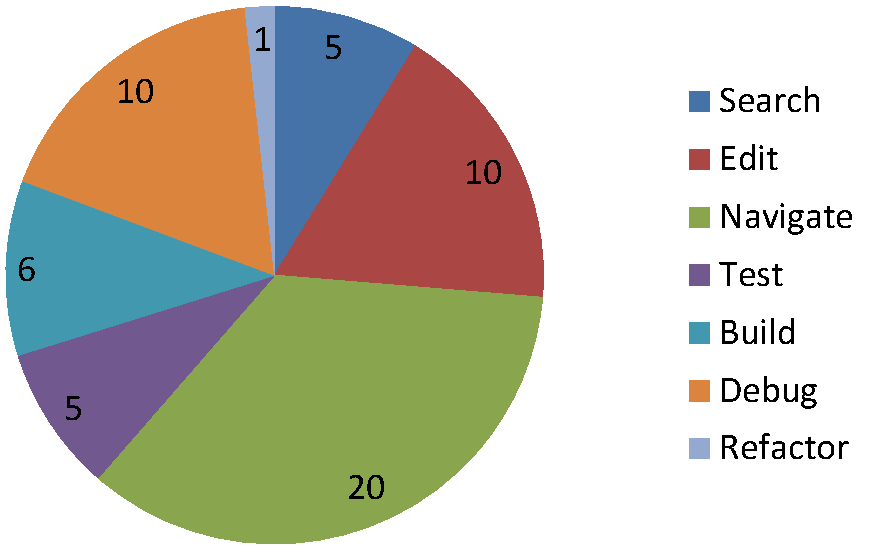
\includegraphics[width=0.5\columnwidth]{26Snipes_activityCategorization.pdf}
\caption{Categorized Log Events with Search Category}
\label{fig:category}
\end{figure*}


\subsection{Sequence Analysis}

%intro to sequence analysis
Magnitude analysis and categorization are both appropriate for answering questions that are simply manifested in the IDE usage log. However, a more powerful way of analyzing activity logs is through sequence analysis, which first breaks the IDE data stream into a number of sequences, according to some criteria, and then reports upon characteristics of each sequence. A sequence in the IDE usage data corresponds to a software engineering task or sub-task accomplished by the developer (e.g. refactoring, looking for a starting point for a maintenance task, etc.), consisting of all of IDE events in a given time span. For instance, answering the question of ``Are developers successful at finding initial points in the code for a software maintenance task?'' requires that the sequence of IDE events corresponding to each maintenance task be identified, before we can perform further analysis using either magnitude or categorization analysis. The granularity of a sequence is determined by the guiding question. For certain questions, we may be interested in a smaller sequences (e.g., searching the code base), while for others we may need to consider a longer time span (e.g., implementing a new feature, fixing a bug). 
According to ~\citeasnoun{Zou-ComanIndustry}, the larger and more complex the task or sub-task to extract, the harder it is for sequence analysis to determine its starting and stopping point in the activity log.

%how difficult or easy is it to determine sequences
In many cases, extracting activity sequences can be challenging as it impossible to know exactly when a developer begins or ends a particular task or sub-task, without understanding the developer's underlying thought process. There are several possibilities in how sequence extraction can be performed, based on the specific question. One possibility is to use sentinels, which are specific actions that indicate the beginning and end of a sequence. For instance, in the context of the code search question mentioned above, submitting a query to the code search tool begins a sequence, while performing an edit or structural navigation (e.g., following the call graph) ends the sequence. Another possibility is to use the passage of time to extract sequences, where time without any activity is used as a signal of task start or finish. Yet another possibility is to use locations in the code base to identify a sequence in the activity log. This is the key insight used in  ~\citename{Coman-TaskIdent}'s algorithm ~\citeyear{Coman-TaskIdent}, which uses periods of activity on the same program elements to represent the core of a task, and time distance between such events to extract sequences corresponding to developer tasks. In laboratory validation studies of this algorithm have shown very high accuracy (80\%) when compared to the ground truth reported by developers. ~\citeasnoun{Zou-ComanIndustry} find that this accuracy may not hold up in an industrial setting, where tasks are longer, code bases are more complex, and developer interruptions are common. Also, the algorithm requires that information regarding program elements is kept in the activity log, which may conflict with many developer's privacy and anonymity requirements.



\begin{figure}
\hrulefill
\begin{verbatim}
Collector Started
2014-02-02 13:46:52 - User submitted query to Find-in-Files
2014-02-02 13:46:56 - Find-in-Files retrieved 121 results
2014-02-02 13:52:21 - User clicked on result 2
2014-02-02 13:58:01 - User clicked on result 8
2014-02-02 13:59:57 - Open caller/callee command 
...
2014-02-02 14:46:52 - User submitted query to Find-in-Files
2014-02-02 14:46:56 - Find-in-Files retrieved 19 results
2014-02-02 15:01:08 - User clicked on result 11
2014-02-02 17:30:12 - User edited code
...
\end{verbatim}
\hrulefill
	\caption{Log File Sequence Example}
	\label{log:logFileSequence}
\end{figure}
%example
We illustrate sequence analysis with the usage log shown in Figure \ref{log:logFileSequence} and the question  ``Are developers successful at finding initial points in the code for a software maintenance task?''
To answer the question, sequence analysis can extract two separate sequences in the log from Figure \ref{log:logFileSequence} by using sentinels indicative of start/end of a code search activity, among other possible sequence identification approaches. Both of the extracted search sequences can be deemed as successful since for each of the queries to the {\tt Find-in-Files} code search tool the developer clicks on a retrieved result, followed by a structured navigation event (open caller/callee) or editing event (developer edited code). Therefore it would seem that the developer is successful at finding initial points in the code for his or her software maintenance task. However, on closer inspection of the second sequence, we observe that there is a large time gap between clicking on a result and editing code. The reason for this time gap is open to interpretation, as the developer may have returned to the previous results, continuing the search session, or have started on a completely new development activity. Certain types of sequence analysis, such as Coman's algorithm, take time into account when identifying sequences, while others, like the sentinel approach used above, do not. Neither of these approaches, however, helps to resolve the origin of ambiguous events, which are left to the reader to characterize.

\subsection{State Model Analysis}

Another way to analyze log data is to view the log as a sequence of events occurring in a state machine.  Using state models, we can quantify the occurrences of repeating actions and describe a usage pattern in statistical analysis.  ~\citeasnoun{nagappan_logs_to_dags_tefse_2011} used sequence analysis to generate a graphical view of a profile of how users interacted with the components of a system from log data.  In state model analysis, the sequential data is converted to nodes and edges of a graph which represents the entire data in states and transitions between them.  A Markov state model provides information about the probability of occurrence of each state and the transitional probability of each activity.   The statistics provided in a Markov state model include the quantity of time and probability for the developer being in each state.  From a given state, the model calculates the probability of each transition to different unique states.  State models answer specific questions such as what is the probability that once a developer searches the code, they edit a code element listed in the find results. Expanding this question, the probability of an entire use case or set of transitions through the usage model, is calculable from the state model.  

State model graphs make it easy to identify the most active states and edges provides information about the important activities in the data set.  As the number of states increases, the Weighted Directed Graph (WDG) becomes more complex and hence difficult to understand.  When this occurs, summarizing the detailed event data into higher-level categories effectively combines the states to get more meaningful information.   For example, classifying events in usage data of similar types into categories results in fewer states with the same number of transitions as the original data.

We generate a state model from a usage log by transforming the serially ordered events in a sequence data to a WDG data structure. Events may repeat many times in the entire log and we have to extract the list of distinct events to represent the entire log as a WDG. In other words, duplicate events are removed and only unique events are represented in the graph. We can abstract the information in the log line to any level, such as, event level, event category level, tool level, or application level. In the sequence data, each event is important as a standalone event, however, in the WDG representation, the importance shifts to adjacent pairs of events. 
%We do this type of a transformation to record the order in which events happened. 
Therefore, each unique event in the sequence data is represented by a unique node in the WDG. 

To understand how to interpret a state model, look at our example graph Figure \ref{op-profile-example}.  We see that an edge exists from one node (head) to another (tail) if there is an occurrence of the event representing the tail node immediately after the event representing the head node in the  log file. For example if event B follows event A in the log file, then there is directed edge from node A to node B in the WDG. The edges are labeled with the number of times this transition has occurred.  For example if B occurs a fifty times after A in the log file, then the edge from node A to node B in the WDG is labeled with 50. Typically, we keep track of the actual count as the weight of the edge, when building the graph. In the graph we display the percentage value as the label. This percentage is proportional to the total number of transitions.  The cumulative probability of out-edges of a node is 1. The transitional probabilities of each out-edge is calculated by dividing the number of transactions of that out-edge with the sum of all outward transactions from that node. We could also store the dynamic parameter information in each log line as a list along the edges. 

As an example, consider a sample log file shown in Figure \ref{samplelogfile} given below and the corresponding state model graph in Figure \ref{op-profile-example}. Intuitively you can see how the state model represents the log states and transitions between them in the sequence of events.  

\begin{figure}
\hrulefill
\begin{verbatim}
2013-03-21 18:18:32Z,A
2013-03-21 18:18:33Z,B
2013-03-21 18:20:49Z,C
2013-03-21 18:20:50Z,A
2013-03-21 18:20:56Z,B
2013-03-21 18:20:57Z,A
2013-03-21 18:21:08Z,C
2013-03-21 18:21:08Z,D
2013-03-21 18:21:08Z,E
2013-03-21 18:21:08Z,A
\end{verbatim}
\hrulefill
\caption{Sample Log File to Convert to State Model}\label{samplelogfile}
\end{figure}

\begin{figure}[h]
  \centering
  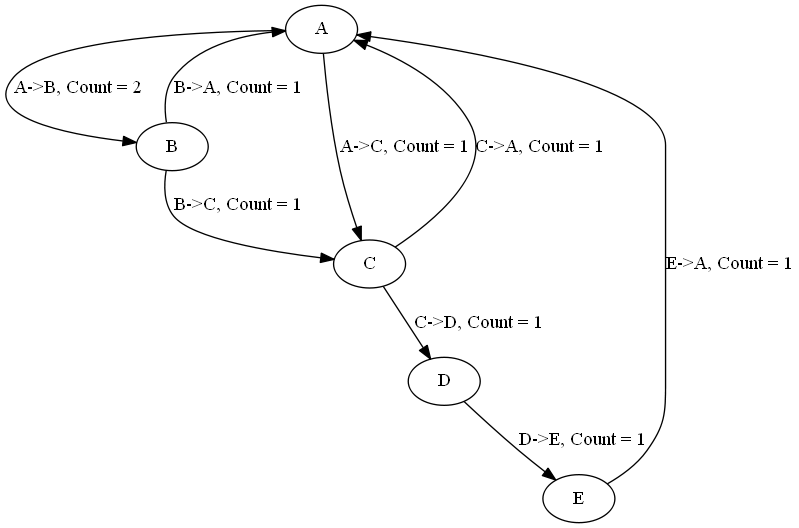
\includegraphics[scale=.40]{26Snipes_op-profile-example.png}
  \caption{Weighted Directed Graph of the Example Log}\label{op-profile-example}
\end{figure}






%the other example is aligned with the sample graph thus better.
%As an example of WDG, consider a simple log file where the activities are separated by commas. $1-2, 2-3, 3-4, 4-5, 5-4, 4-5, 5-4, 4-6, 6-7, 7-5, 5-4, 4-5, 5-4, 4-5, 5-8, 8-9$. The events in the log file are mapped to their corresponding event IDs: $1, 2, 3, 4, 5, 4, 5, 4, 6, 7, 5, 4, 5, 4, 5, 8, 9$. Each node is a unique event. An edge between nodes 1 and 2 signifies that the event 2  appears after event 1  in the log file. The labels on the edges have the actual count and could have the transitional probabilities as well. The transitional probability from node 1 to node 2 is 1.0, whereas the transitional probability from node 4 to node 6 is 0.2.  This is depicted in Fig \ref{op-profile-example}.
 
Converting a log into a state model requires three steps.  We use JUMBL (Java Usage Model Builder) from the Software Quality Research Laboratory (SQRL) of the University of Tennessee.    Details on input formats and JUMBL tools are available on sourceforge.\footnote{\url{http://jumbl.sourceforge.net/}}
\begin{enumerate}
\item
First, convert the log file into a representation for each transition called a sequence based specification. The format for a sequence based specficicaiton in csv files is described in the JUMBL user guide. This representation contains the following information with one row for each transition :
\begin{itemize}
\item State transition
\item Count of transitions
\item Total time elapsed
\item State In information
\item State Out information
\end{itemize}

\item
After importing the sequence based spec, JUMBL can write out the representation of a state model as a TML script or several other formats including GML (Graph Modeling Language) that graph tools can import.  The TML  has information about the nodes, the out edges from each node along with the number of transitions from each node to another. The corresponding graph for the usage log example is depicted in Figure \ref{op-profile-example}
\end{enumerate}


Using state models, a sequence data with hundreds of thousands of lines can be quickly converted to more meaningful graphical representation using this method. Once the TML file is generated, we can use JUMBL to find out the state probabilities of each states. Using the state probability and the usage patterns we can draw conclusions about the occupancy of individual states and the use cases that involve transitions through several states.

%Trying this on without the following examples.  They don't really add much and raise more questions than they answer.  I hope reference take care of the how to in this case.


%
%\begin{figure}
%\label{sampleTML}
%\hrulefill
%\begin{verbatim}
%($ fill(1) $)
%model testlog
%//use this before each transition to show probability ($0.10$)
%
%source [A]
%($2$)"Count=2 (A->B), TimeElapsed= 7secs" [B]
%($1$)"Count=1 (A->C), TimeElapsed= 11secs" [C]
%
%[B]
%($1$)"Count=1 (B->C), TimeElapsed= 136secs" [C]
%($1$)"Count=1 (B->A), TimeElapsed= 1secs" [A]
%
%[C]
%($1$)"Count=1 (C->A), TimeElapsed= 1secs" [A]
%($1$)"Count=1 (C->D)" [D]
%
%[D]
%($1$)"Count=1 (D->E)" [E]
%
%[E]
%($1$)"Count=1 (E->A)" [A]
%
%
%"exit" [Exit]
%
%end 
%\end{verbatim}
%\hrulefill
%\caption{Sample TML for a State Model}
%\end{figure}



%%I commented these out because they were out in space in the document and not well supported by the text.  You probably cut the text because of other comments.  Anyhow does it make sense to stick with one WDG example based on the state model shown in text above?  Seems OK to me so far. 

 
\subsection{The Critical Incident Technique (CIT)}

The Critical Incident Technique (CIT) is a general methodology for improving a
process or system with respect to a set of objectives. CIT prescribes a
systematic study of the \emph{critical incidents}. Critical incidents are
\emph{positive} or \emph{negative} events that have a significant effect on the
objectives.

CIT was developed and published in its current form by Flanagan in
1954~\cite{Flanagan1954CIT}. Nevertheless, it is believed that the technique was
introduced even earlier by Galton (circa 1930). Variations of CIT have been
widely used in Human Factors~\cite{ShattuckWoods1994CIT}.

~\citeasnoun{DelGaldo1986CIT} applied CIT to Human-Computer Interaction (HCI) as part
of evaluating the documentation of a conferencing system.
They asked the study participants to perform a task and report any incident that
they ran into. The researchers observed the participants during the study,
analyzed the reported incidents, and proposed improvements to the documentation
accordingly.

In the context of IDEs, ~\citeasnoun{VakilianJohnson2014Alternate} adapted CIT to automated
refactorings. The goal of this study was to
identify the usability problems of automated refactorings by analyzing
refactoring usage data. The researchers found that certain events such as
cancellations, reported messages, and repeated invocations are likely indicators
of the usability problems of automated refactorings. By locating these events in
the usage data and analyzing their nearby events, the researchers were able to
identify 15 usability problems of the Eclipse refactoring tool. For instance,
the usage data indicated that six participants invoked the Move Instance Method
refactoring for a total of 16 times but none finished the refactoring
successfully. In all cases, the participants either canceled the refactoring or
could not proceed because of an error that the refactoring tool reported. By
inspecting these critical incidents, the researchers were able to infer two
usability problems related to Move Instance Method.

To apply CIT on a set of usage data, you should follow several steps. First,
identify the objectives. Finding usability problems is only one example.
Second, identify a set of events that may be critical incidents. These are
events they may have significant effects on your objectives. Usually, the
negative critical incidents, which may have negative effects on the objectives,
are better indicators of problems than the positive ones. Third, identify the
critical incidents in your usage data. Fourth, collect sufficient contextual
information to interpret the critical incidents. This may include events that
have occurred in close time proximity to the critical incidents. You may even
have to interview the developers or ask them to report their explanations of the
incidents during the study. Although the developer reports may be short or
incomplete, they can provide more insight about the nature of the problems.
Finally, evaluate the effectiveness of the critical incidents and revisit the
steps above. The process that we described for applying CIT on usage data is
iterative in nature. That is, it is natural to go back to a previous step from
each step.

\label{sec:IncludingOtherSources}
\subsection{Including Data From Other Sources}


Other data sources, such as developer feedback, task descriptions, change histories can provide context for usage data and yield new opportunities for supporting developers. In this section, we briefly outline some related work in this area.

\subsubsection{Developer Feedback}

Usage data collection can be augmented by explicit developer feedback to establish a ground truth. For instance, if you want to understand a developer's opinion of a tool or his or her purpose for using an IDE feature, it is best to ask about it. A post-analysis interview can shed light on your observations and confirm your analysis or point out different aspects.

Information on a developer's activities can provide an additional rational to the usage data and explain the developer's actions. Asking questions on how well the developer knows the code he or she is working on can explain a developer's navigation patterns and usage of code search~\citeaffixed{SnipesExperiencesGamifyingSoftwareDevelopment}{e.g.,}, while questions on the task, e.g., implementing a new feature versus fixing a bug, can explain other characteristics, such as the amount of editing versus testing.

\subsubsection{Tasks}

As mentioned above, Mylin is a popular extension to the Eclipse IDE that supports task
management, reducing the effort for a developer to switch between
tasks and maintaining relevant information for each
task~\cite{Kersten-Mylyn}. In the context of a specific task, Mylin
collects usage data in order to compute a degree-of-interest (DOI)
value for each program element, which represents the interest the
developer has in the program element for the task at hand. Program elements that a developer interacted with frequently and recently have a higher DOI value. Using these calculated DOI values, Mylyn highlights the elements relevant for the current task and filters unnecessary information from common views in the IDE. 

\subsubsection{Change History}

The FastDash tool by ~\citeasnoun{FastDash} enables real-time awareness of other developers'
actions (e.g., focus or edits to a specific file) by utilizing usage
data in concert with the source files and
directories. FastDash's purpose is to reduce faults
caused by lack of communication and lack of awareness of activities
that other developers are performing on the same code base. The tool
highlights other developer's activity as it is occurring using a
sophisticated dashboard on the developer's screen or on a team's dashboard.




